\documentclass[12pt]{report}                  % Times New Roman, 12pt
% \usepackage{gscale_thesis_singlespace} % Single spaced thesis
\usepackage{gscale_thesis_doublespace} % Double spaced thesis
\usepackage{fancyheadings}                   % Header and footer styling
\usepackage{natbib}                               % Bibliography formatting
\usepackage{setspace}                           % Allows double spacing but skips headers/footers
\title{Assurance for Machine Learning systems}
\halftitle{Assurance for Machine Learning systems} % 60 Characters Max. Including Spaces

\author{Milad Hassani}
\shortauthor{M. Hassani} % Used for page header

\dept{computing and software} % The department you are part of; Must be all lower case
\field{computer science} % What field your thesis is in

\prevdegreeone{Ph.D. (Computer Science),\\ McMaster University, Hamilton, Canada}
\prevdegreetwo{Ph.D.} % Just your degree's field

\submitdate{June 2021}
\copyrightyear{2021}

\principaladviser{Dr. Richard Paige} % Your Supervisor
                                % LaTeX variables for preface pages/headers
\setcounter{tocdepth}{1}                        % Limits the TOC to chapter and section names

% Additional packages
\usepackage{graphicx}                                   % Allows the inclusion of figures
\usepackage{subcaption}                               % Allows captions to be added to subfigures
\usepackage[justification=centering]{caption} % Centres caption text
\usepackage[hidelinks]{hyperref}                    % Linking to LaTeX labels and external URLs
\usepackage{array}                                        % Used for table formatting
\newcolumntype{P}[1]{>{\raggedright\let\newline\\\arraybackslash\hspace{0pt}}m{#1}}
\usepackage{booktabs}                                 % Fancy-style tables
\usepackage{longtable}                                 % Allows for tables that are more than one page long
\usepackage{float}                                         % Better figure placement control
\usepackage{enumerate}   
\usepackage[shortlabels]{enumitem}                            % Numbered lists 
\usepackage[shortcuts]{extdash}                  % Allows manual hyphenation of hyphenated words
\usepackage{amsmath}                                % Non-standard math symbols
\usepackage{amsfonts}                                % Extended fonts for 
%mathematics
\usepackage{xcolor}
\usepackage{csquotes}                            % Allows quotes
\usepackage{multirow}
\numberwithin{equation}{section}                 % Numbers equations based on their section

% ********************************
\begin{document}
\beforepreface                                         % Half title page, title page, declaration page   
%   \prefacesection{Lay Abstract}

A lay abstract of not more 150 words must be included explaining the key goals and contributions of the thesis in lay terms that is accessible to the general public.                                  % Lay Abstract
  \prefacesection{Abstract}

Machine Learning (ML) has become one of the fastest growing fields of science in recent years. The theories and technologies underpinning ML are used in a vast number of industrial and scientific applications, including banking, security, automotive and healthcare. Although it is becoming more prevalent to use ML technologies in safety critical settings such as healthcare and aerospace, there is still a significant need to assure safety of such systems. In this report, we will first take a look at the foundations of ML and safety. Next we review some of the methods currently developed for safety assurance in ML. We present these methods using a conceptual model based on four stages of ML: Data Management, Model Training, Model Verification and Model Deployment. We identify some of the open research areas associated with each stage.                                       % Abstract
  %%\thispagestyle{empty}
\null\vfill
\begin{center}
%\textbf{Dedications}
%\linebreak
\textsl{Your Dedication \\ Optional second line}
\end{center}
\vfill
                                      % Dedication
  %\prefacesection{Acknowledgements}

Acknowledgements go here.                 % Acknowledgements
  \referencepageswithnotations{notation} % Table of Contents, List of Figures, List of Tables, Notations
  %\referencepages                                 % No notations version (choose one)
\afterpreface                      
  
  
  \chapter{Introduction}

With new developments in Artificial Intelligence (AI) and ML, a growing number of research projects in this field and many companies have started utilizing these methods.
ML methods are also used in many safety critical applications such as Autonomous Vehicles (AVs) and healthcare applications. Therefore, it is very important to have a clear perspective of the safety of such methods in these applications.

In some applications, an erroneous outcome of the ML model has a harmful impact on many lives, for example in medical diagnosis \cite{Foster2014}, loan approval \cite{Lessmann2015}, autonomous vehicles \cite{koopman2016challenges}, and prison sentencing \cite{Berk2015}.
Despite the numerous research papers in this subject, there is still a need to delve deeper and understand the behavior of ML systems in safety critical applications.

One major drawback in using ML algorithms is that they are often treated as a black box and hence, using safety procedures for these methods is sometimes inapplicable \cite{Schwalbe2020}. In a review of automotive software safety methods \cite{Salay2017}, an analysis of ISO-26262 part-6 methods was performed with respect to safety of ML models. This assessment shows that about 40\% of software safety methods do not apply to ML models \cite{Salay2017}.


Safety specifications often assume that behavior of a component is fully specified. Since the training sets used in ML methods are not necessarily complete, they violate this assumption, and some parts of the specification becomes not applicable to the ML components \cite{Salay2017}. 
Most widely used ML frameworks such as Tensorflow \cite{Abadi2016Tensor} \textcolor{red}{are Pytorch and Caffe using a model driven approach??????} and Theano \cite{Al-Rfou} employ a model driven approach in problem solving. Although model driven engineering approach has been successful in safety critical applications such as Automotive industry, the ML models cannot be guaranteed to operate in a safe manner. 

There are two approaches with respect to ML and safety, first is to study safety of ML methods, algorithms, and processes and the second is to use ML methods to improve pre-existing safety assurance procedures.
We will initially follow the first approach and review the literature for the methods applied to standardize and measure the safety of ML methods.

There are inherent performance metrics related to ML methods, such as accuracy and robustness, which can affect their applicability in safety critical applications. ML models can also be dependent to the domain they are trained \cite{Ganin2015}. In addition, other perturbations such as noise, natural and imaging artifacts can cause ML models to function less accurately \cite{Hendrycks2019}.

In this report we will first explore basics of ML in Chapter \ref{chap:ML}. Then in Chapter \ref{chap:safety} we review definition of safety and how assurance cases are structured. Finally in Chapter \ref{chap:literature} we survey the literature on ML assurance and identify some of the open challenges in this area.                  
        \setcounter{figure}{0}
        \setcounter{equation}{0}
        \setcounter{table}{0}
        
  \chapter{Machine Learning}
\section{Definition}
Machine learning algorithms can extract patterns and learn from data \cite{IanGoodfellow2016}. A brief definition of learning can be given as \cite{mitchell1997machine}
\begin{displayquote}[][]
    "A computer program is said to learn from experience \textit{E} with respect to some class of tasks \textit{T} and performance measure \textit{P}, if its performance at tasks in \textit{T}, as measured by \textit{P}, improves with experience \textit{E}."
\end{displayquote}

A task is the main objective of using an ML algorithm. For example, in an autonomous vehicle, driving the car is the task. A task is not the process of learning. Learning is used as a means to achieve an ability to accomplish a task \cite{IanGoodfellow2016}. With developments in ML methods, they have been applied to different tasks, some examples of tasks are classification, regression, transcription, machine translation, denoising \cite{IanGoodfellow2016}.

The performance measure is used to quantify how successfully a task is accomplished, equivalently, number of erroneous outputs could be used as a way of indicating a method's performance. 

Based on the above-stated definition, the ML algorithm undergoes an experience in the process of learning. This experience is generally classified into \textbf{unsupervised}, \textbf{supervised} and \textbf{reinforcement} learning.

\section{Learning types}

Unsupervised learning finds the properties of the overall structure of the dataset. Clustering as an example of unsupervised learning, finds clusters within a dataset and assigns each data-point to one of them.\\In supervised learning, on the other hand, data-points that the learning algorithm experiences have a label. This label acts as a guide for the ML algorithm. The term supervised arises from the fact that the labels instruct the algorithm what to do. Labels are unavailable in unsupervised learning and the ML system is responsible to make sense of the data independently \cite{IanGoodfellow2016}. 

Reinforcement learning (RL) algorithms experience an environment instead of a fixed dataset. The algorithm should learn how to maximize a reward function by taking an appropriate action \cite{sutton1992introduction}. The learner discovers this appropriate action by trying different actions and observing the value of the reward function. Actions not only affect the immediate reward, but can also change next actions' rewards. Trial and error search and delayed reward are two main characteristics of RL.\\The learner, also known as the agent in RL terms, should have the capability to sense the state of the environment, take actions that can alter the state and also have a goal to reach by taking actions. These three aspects are included in the reward function used by the agent \cite{sutton1992introduction} \textcolor{red}{more about Deep RL?}

\section{Data in ML}

Evidently, ML algorithms need data to learn and function. A dataset can be described as a \textbf{design matrix}. Every row in the matrix contains an example, also known as data-point, and each column is a feature. Iris dataset is one of the first ones used in statistics and ML \cite{Fischer1936Iris}. This dataset is comprised of 150 examples which have 4 features each. One example corresponds to one individual plant. Sepal length, sepal width, petal length and petal width are recorded as features of each plant \cite{Fischer1936Iris}.
This means that if $X$ is the matrix, we can say $\mathbf{X} \in R^{150 \times 4}$

The ML model will ultimately be deployed and used in a real world situation, hence, we are interested in how well an ML model performs on the data it has not seen before, this is also known as \textbf{generalization}. A portion of dataset is therefore not used in the training process and reserved as a \textbf{test set}. The data used in the training process is accordingly referred to as the \textbf{training set} \cite{IanGoodfellow2016}. 

In some cases, the training and test datasets might be limited in size and to have a better generalization, it is necessary to use as much of the data for training as possible. In other words, there will be less data available to estimate the performance of the model. One solution for this situation is \textbf{cross-validation}. The entire dataset is split into ${S}$ subsets. In each run, ${S - 1}$ subsets are used for training and one remaining subset is the test set. For the next run, a different test set is selected \cite{bishop2006pattern}. Figure \ref{fig:crossv} shows selection of subset for ${S = 4}$.

\begin{figure}
    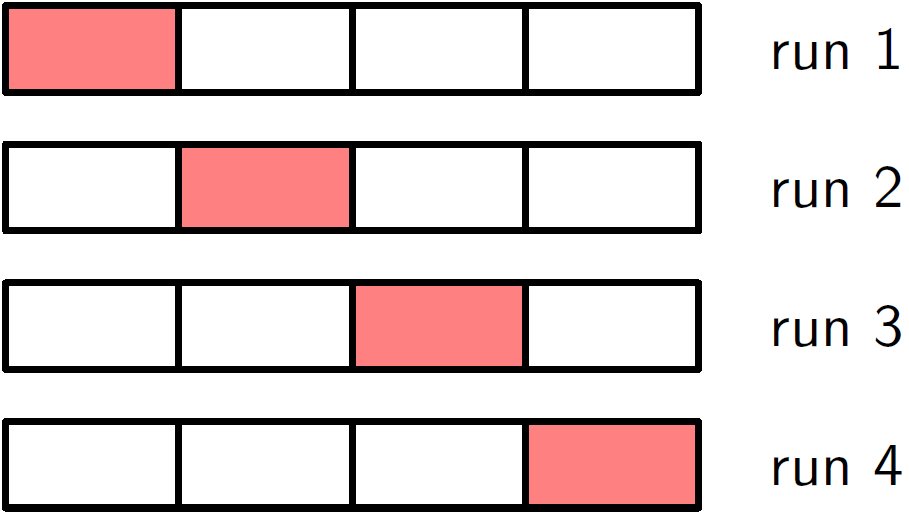
\includegraphics[width=0.5\linewidth ]{figures/crossv.png}
    \centering
    \caption{Cross validation for S=4 \cite{bishop2006pattern}.}
    \label{fig:crossv}
\end{figure}



\textcolor{red}{add about neural networks}\\                  
       \setcounter{figure}{0}
       \setcounter{equation}{0}
       \setcounter{table}{0}

  \chapter{Safety and assurance}

In \cite{Amodei}, five major research problems associated with unsafe behavior of ML models is presented. They can be summarized as
\begin{enumerate}
	\item Avoiding Negative Side Effects: How to ensure that the model will not disturb the environment while pursuing its goals, e.g. can a cleaning robot knock over a vase because it can clean faster by doing so? Can we do this without manually specifying everything the robot should not disturb \cite{Amodei}?
	
	\item Avoiding Reward Hacking: How to ensure that the model does not avoid situations to achieve a higher reward. For example, if we reward the robot for achieving an environment free of messes, it might disable its vision so that it won’t find any messes, or cover over messes with materials it can’t see through, or simply hide when humans are around so they can’t tell it about new types of messes \cite{Amodei}. 
	
	\item Scalable Oversight: How to ensure the model respects the parts of the objective function that are expensive to evaluate and makes a safe approximation of these parts. 
	For example, in the cleaning robot example, if the user is happy with the cleaning quality is an expensive objective function, but it can be approximated to presence of any dirt on the floor when the user arrives \cite{Amodei}. 
	
	\item Safe Exploration: How to ensure that the ML model explorations are safe. For example, the robot should experiment with mopping strategies, but putting a wet mop in an electrical outlet is a very bad idea \cite{Amodei}. 
	
	\item Robustness to Distributional Shift: How to ensure that the model performs robustly if the environment shifts from the training environment. For example, strategies a cleaning robot learns for cleaning an office might be dangerous on a factory work-floor \cite{Amodei}.

\end{enumerate}                  
       \setcounter{figure}{0}
       \setcounter{equation}{0}
       \setcounter{table}{0}

  \chapter{Literature Review}
\label{chap:literature}

In this chapter we will briefly review some of the literature about the safety of ML methods and identify major research questions in this area. 
Today, ML is used in variety of applications with varying safety requirements. This diverse portfolio includes smart phones \cite{smartphone2012}, cars \cite{Levinson2011}, surgical equipment \cite{Egert2020}, construction industry \cite{bilal2020} and many more. A fault in an ML system, e.g. a misclassification, has different repercussions in each application. An out of focus image taken by a camera can be easily remedied, but a malfunction in a surgical equipment could be fatal and result in an irreversible situation. Therefore, assuring safety is an essential part of the design process for these applications.

One major issue in safety assurance for ML is guaranteeing that the training data is complete and relevant. Data used in the operational stage is by definition relevant, however, training data may not reflect all possible situations that the learning algorithm needs to be exposed to. On the other hand, the operational environment may change and the training data may diminish in relevancy. As discussed in detail later in this chapter, assuring completeness and relevancy is challenging and may not always be feasible. 

% \textcolor{blue}{IDEA: Creating a map of ML. Listing all successful applicaitons of ML in industry for example.}
% 
\textcolor{red}{As this part is mostly concerned with RL I should put it in a separate subsection}
In \cite{Amodei2016}, five major research problems associated with unsafe behavior of ML models is presented. They can be summarized as
\begin{enumerate}
	\item Avoiding Negative Side Effects: How to ensure that the model will not disturb the environment while pursuing its goals, e.g. can a cleaning robot knock over a vase because it can clean faster by doing so? Can we do this without manually specifying everything the robot should not disturb.
	
	\item Avoiding Reward Hacking: How to ensure that the model does not avoid situations to achieve a higher reward. For example, if we reward the robot for achieving an environment free of messes, it might disable its vision so that it won’t find any messes, or cover over messes with materials it can’t see through, or simply hide when humans are around so they can’t tell it about new types of messes.
	
	\item Scalable Oversight: How to ensure the model respects the parts of the objective function that are expensive to evaluate and makes a safe approximation of these parts. 
	For example, in the cleaning robot example, if the user is happy with the cleaning quality is an expensive objective function, but it can be approximated to presence of any dirt on the floor when the user arrives.
	
	\item Safe Exploration: How to ensure that the ML model explorations are safe. For example, the robot should experiment with mopping strategies, but putting a wet mop in an electrical outlet is a very bad idea.
	
	\item Robustness to Distributional Shift: How to ensure that the model performs robustly if the environment shifts from the training environment. For example, strategies a cleaning robot learns for cleaning an office might be dangerous on a factory work-floor.

\end{enumerate}

% Some of the above 
\section{Machine Learning lifecycle}

To obtain assurance for ML systems it is essential to understand the ML lifecycle and how to analyze safety in each step. In this section we will first introduce these steps and review some of the safety measures for each step. This lifecycle follows a spiral process model, i.e., the stages are iteratively repeated to actively reduce risk \cite{Boehm2000}. ML lifecycle is comprised of four stages \cite{Ashmore2021} 

\subsection{Data Management}
\label{sub:DM}
This stage involves collecting, preprocessing, augmenting and initial analysis of data. The training and validation datasets are also prepared in this step.
From assurance perspective, the data collected in this step should be
\begin{itemize}
    \item Relevant: The dataset should be relevant to the desired functionality of the final model. For example a dataset of handwritten letters in Japanese language cannot be used for English language. In many cases, a pre-existing dataset will be used to train the model. This dataset should be obtained from trusted sources with an encrypted transmission medium. An attacker can add irrelevant samples into the training dataset to make the final model behave in a specified way for particular inputs \cite{Chen2017}. The irrelevant data injected in the dataset is called a backdoor \cite{Chen2017} Despite early efforts in detecting backdoors in face recognition \cite{Wang2019} finding a general solution is still an open challenge.
    \item Complete: The features of a dataset should not have unintended correlations that can confuse the classifier. For example, if a classifier is trained on pictures of wolves and huskies, and all wolves have snow in the background, it may be concluded that snow in the background means a wolf \cite{Ribeiro2016}. In this case the dataset is not complete because it does not include pictures of wolves with different backgrounds. Exploratory Data Analysis (EDA), is an important step in examining completeness of a dataset. It is also important to identify how the data points are distributed in the input sample space, measures such as gap ratio \cite{Teramoto} can be used to evaluate uniformity.
    \item Balanced: For classification problems, it can happen that one class has significantly more data-points in the training set than the others and thus, classifier has more exposure to that class. 
    \item Accurate: This property considers factors like sensor accuracy, correctness of data collection and processing method. In the case of supervised learning, labels' accuracy is important. The data collection process should be documented to identify potential inaccuracies \cite{Ashmore2021}.
\end{itemize} 

\subsection{Model Learning}
In this stage of the ML lifecycle, the type of the model and its hyper-parameters are selected. For some ML applications, the dataset is very large or the model structure is complex and therefore, the learning process needs considerable amount of computational power. In these cases, it is reasonable to take advantage of a previously trained model and adapt it to our needs by re-training only the parts that are different from the other application. This process is called \textit{transfer learning} \cite{IanGoodfellow2016}. If there is a need to do transfer learning, it will be decided at this stage and finally the learning process starts using the train dataset obtained in previous stage.
In order to have a clear view of the model in safety related aspects, the final model should be \cite{Ashmore2021}  
\begin{itemize}
    \item Performant: As a requirement for a safer model, it should have a justifiable performance according to the measures introduced in \autoref{chap:ML}.
    \item Robust: The model should be able to perform as well on the unseen data as the training data,i.e., generalizes well to be considered robust. Data augmentation is one of the techniques to increase generalization \cite{Ko2015}. 
    \item Reusable: Using transfer learning can help to use the assurance evidence of the original model, provided that the transfer learning is performed in the right context for the source and destination models. However, reusing models comes with the risk that safety issues propagates to the destination model too 
    \item Interpretable: This property shows how much the decisions made by the model are explainable and thus helps to analyze the safety of such decisions. 
\end{itemize}

\subsection{Model Verification and Validation} 
The black swan problem expounds one of the major challenges in validating ML models. A system or a person could incorrectly conclude from abundance of training data samples that common observations are true \cite{koopman2016challenges}. A model which has only seen white swans, may infer that all swans are white and ignore the fact that there are black swans \cite{taleb2007the}. One major challenge is thus making sure that the model works well, i.e., satisfies its requirements, on the data it has not seen before which is also known as generalization. If the model fails in this stage, the process will go back to Data Management or Model Learning steps. Model verification involves requirements encoding, test-based verification and formal verification. The verification stage should be \cite{Ashmore2021}
\begin{itemize}
    \item Comprehensive: Model verification should ensure that all the requirements of the system and also intended goals of the previous stages of ML lifecycle, i.e., data management and model learning, are covered.
    \item Contextually relevant: Verification process should be relevant to the intended use of the ML model. For example an ML model used in autonomous vehicles, we are more concerned about how changes in the environment will affect model's performance and thus, how robust is the model with changes in weather rather than the changes in image quality. 
    \item Comprehensible: Verification results should be understandable for the users. Requirement violations should be clearly expressed in such a way that the cause of it can be identified and fixed \cite{Ashmore2021}. Ideally, the results should also include any black swan biases present in the model \cite{koopman2016challenges}.
\end{itemize}

\subsection{Model Deployment} 
Preparing the ML model to be used in the final application. Activities in stage includes integration, monitoring and updating. To assure safety of this stage of ML lifecycle, the ML model should have the following properties

\begin{itemize}
    \item Fit-for-Purpose: The difference in hardware can cause performance differences between ML stages. Also, each distinct hardware setting where a model is deployed can affect model's performance. For a model to be fit for purpose, the performance seen in the previous stages should be carried over to the deployment phase. 
    \item Tolerable: The system should be able to tolerate occasional incorrect outputs of the ML model. To accommodate this, the host system should be able to identify the incorrect outputs and to replace them with a safe value so that the system continues the normal processing activities.
    \item Adaptable: Deployed models are in many cases needed to be updated due to variety of reasons including operational, legislative or environmental changes. This property indicates how safe is the process of updating. 
\end{itemize}

\section{Open challenges in ML assurance}
Using an ML component in a system poses several challenges in each step of the ML lifecycle. In the data management step, further research is needed to guarantee security of data and its fitness for the purpose. Although a vast amount of research has been conducted in the model learning stage, there is still a need to further study hyper-parameter selection. In addition, with recent successes in transfer learning, there is still need for more research in assuring safety in this area. Furthermore, safety assurance requires ML models to be reusable and interpretable. Model verification assurance is mainly accomplished using test-based and verifications. However, there is still a need to develop methods to encode model requirements into proper and formal tests. In model deployment stage, there is no explicit equivalent for updating models in software engineering world, therefore, there is a need to devise assurance methods for adaptable safety-critical systems \cite{Ashmore2021}.

In some applications requirements for a safe ML system reinforce each other. For example, accuracy in data management stage will most likely result in more performant model. However, in some cases, there is a trade-off between requirements, an explainable model is probably more exposable to cyberattack \cite{Ashmore2021}. In spite of attempts to address this issue \cite{Johnson2019}, more research is required to adapt these concepts to ML.                    
       \setcounter{figure}{0}
       \setcounter{equation}{0}
       \setcounter{table}{0}

  \chapter{Conclusion}

In this report we first started with the basidc definitions and principals of machine learning and safety assurance concept and eplored some of the fundamentals in both areas in Chapter \ref{chap:ML} and Chapter \ref{chap:safety} we also glanced currently trending research in these areas. Finally, in Chapter \ref{chap:literature} we reviewed some of the literature in assurance of ML systems and some of the open challenges and research questions in this field. 

\textcolor{red}{State some of the major open challenges I found,}
        \setcounter{figure}{0}
        \setcounter{equation}{0}
        \setcounter{table}{0}

% \begin{appendix}
% 	\chapter{Your Appendix}
\label{appendix_a}

Your appendix goes here.

% 		\setcounter{figure}{0}
% 		\setcounter{equation}{0}
% 		\setcounter{table}{0}
		
% 	\chapter{Long Tables}
\label{appendix_b}

This appendix demonstrates the use of a long table that spans multiple pages.

\begin{center}
\begin{longtable}{P{3cm}P{3cm}P{2.5cm}P{3.5cm}}
\toprule
\hline
\textbf{Col A} & \textbf{Col B} & \textbf{Col C} & \textbf{Col D} \\ \midrule

\endfirsthead
\multicolumn{4}{c}{\textit{Continued from previous page}} \\ \hline
\textbf{Col A} & \textbf{Col B} & \textbf{Col C} & \textbf{Col D} \\ \hline
\endhead
\hline \multicolumn{4}{r}{\textit{Continued on the next page}} \\
\endfoot
\hline
\endlastfoot

A & B & C & D \\ \midrule

A & B & C & D \\ \midrule

A & B & C & D \\ \midrule

A & B & C & D \\ \midrule

A & B & C & D \\ \midrule

A & B & C & D \\ \midrule

A & B & C & D \\ \midrule

A & B & C & D \\ \midrule

A & B & C & D \\ \midrule

A & B & C & D \\ \midrule

A & B & C & D \\ \midrule

A & B & C & D \\ \midrule

A & B & C & D \\ \midrule

A & B & C & D \\ \midrule

A & B & C & D \\ \midrule

A & B & C & D \\ \midrule

A & B & C & D \\ \midrule

A & B & C & D \\ \midrule

A & B & C & D \\ \midrule

A & B & C & D \\ \midrule

\hline
\end{longtable}
\end{center}

% 		\setcounter{figure}{0}
% 		\setcounter{equation}{0}
% 		\setcounter{table}{0}
% \end{appendix}

% The bibliography is set up to allow for multiple bib files
\bibliographystyle{plain}
\bibliography{library}

\label{NumDocumentPages}

\end{document}
% ********************************
